\section{Grunnleggende}
\subsection{Starte programmet}
\subsubsection*{Metode 1}
\begin{enumerate}
	\item Trykk på konfigurasjon på skrivebordet.
  \item Velg Importer konfigurasjon fra katalog og finn filen ''ProsjektAIM2014\_X\_EDIT\_YYYY'' der X er versjon, og YYYY er dato på formen ddmm.
  \item Trykk på resetknappen på RCU500 i AIM1000-skapet.
	\item Trykk på ''StartAIM.bat'' på skrivebordet slik at programmet starter opp. Logg deretter inn med brukernavn: Simrad og passord: simrad. 
\end{enumerate}

\subsubsection*{Metode 2}
\begin{enumerate}
  \item Siden lab-pcen er konfigurert til prosjektet, kan man benytte seg av filen ''StartAIM\_OS1.bat'' som ligger på skrivebordet.
  \item Logg inn med brukernavn: Simrad og passord: simrad.
\end{enumerate}

\subsection{Operatørpanel}
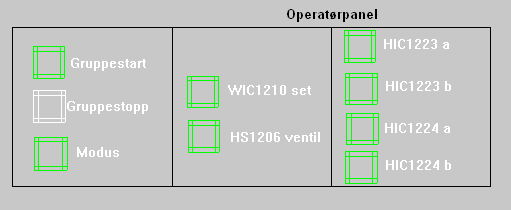
\includegraphics[]{operatorpanel.png} \\
Et overordnet panel for automatisk styring av systemet. Til venstre settes gruppestart og -stopp, og Auto/Manuell modus. I den midtre og høyre delen settes referansepunktet for PID-regulatoren, samt knapper for å åpne og lukke ventilene.
 

\subsection{Starte systemet}
\subsubsection*{Normal start}
For å starte systemet i gruppestart. Sørg for at modulene står i ekstern modus, og systemet i AUTO. 
\subsubsection*{Start etter manuell stopp}
Hvis modulen står i intern modus, må den startes internt. Står modulen i eksternmodus skal den startes fra operatørpanelet. 

\subsection{Stoppe systemet}
\subsubsection*{Gruppestopp}
For å stoppe hele systemet eksternt, benytt gruppestopp. Det er forutsatt at alle modulene står i ekstern modus, samt at systemet står i AUTO. 
\subsubsection*{Manuell stopp}
Hvis motoren står i intern modus, kan man stoppe hver enkelt modul manuelt etter de spesifike krav til hver modul. 

\newpage

\section{Systemoversikt}

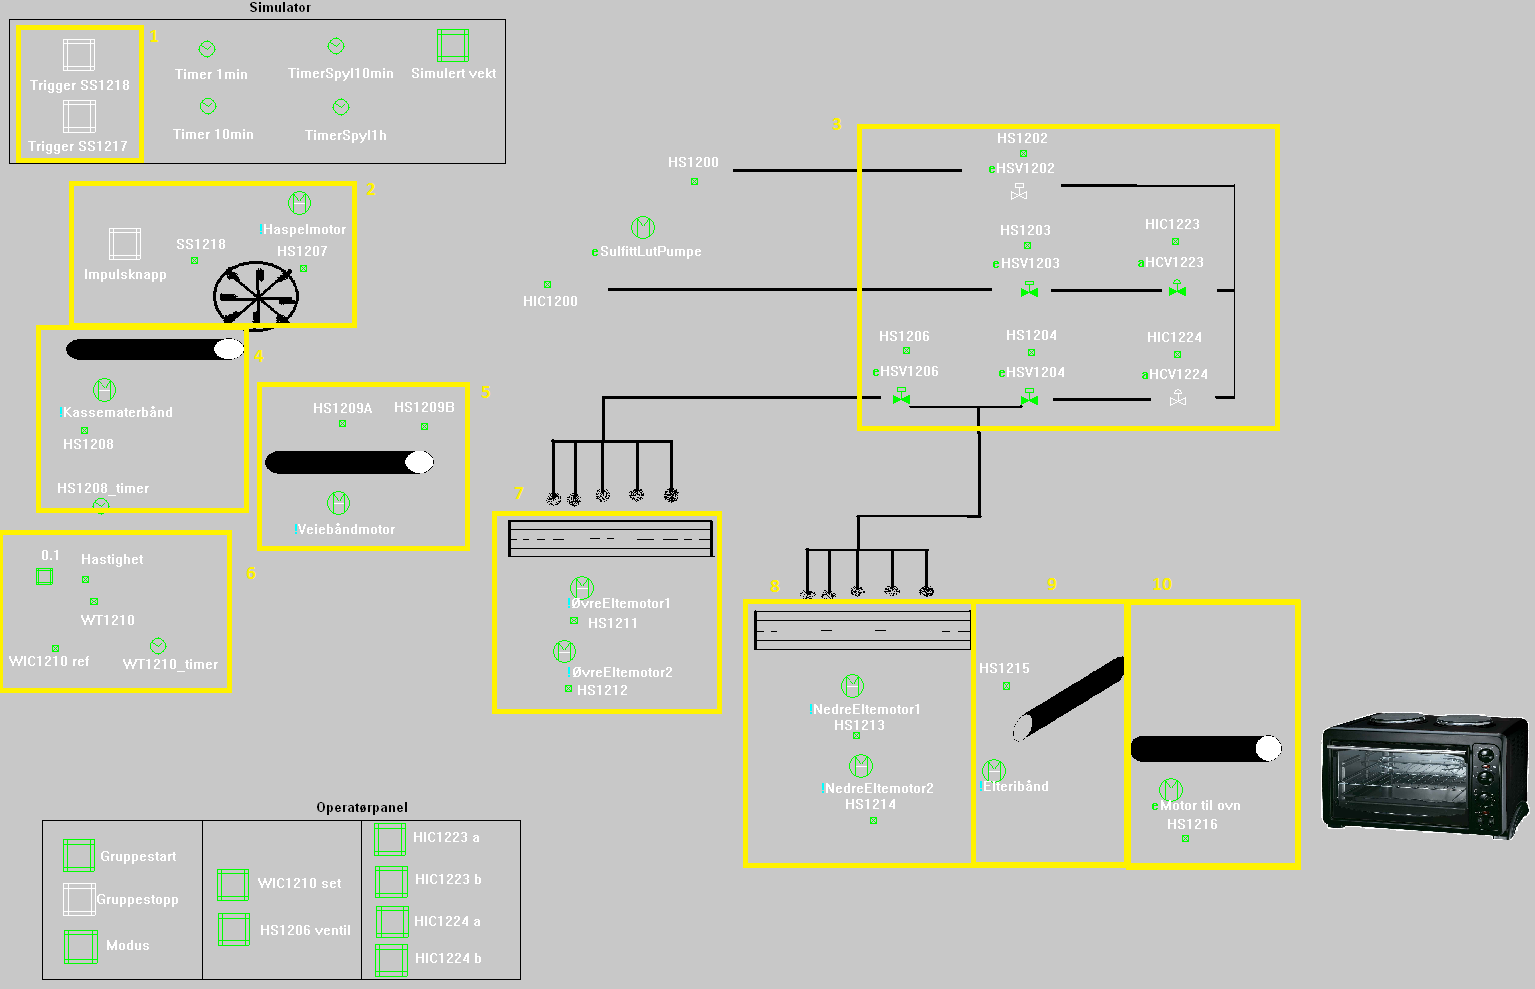
\includegraphics[width=\textwidth]{oversikt.png}

\begin{enumerate}
  \item Trigger hastighetsvakt for haspel og rørkammerbånd
  \item Haspelmodul
  \item Ventilsystem for tilførsel av vann og sulfittlut
  \item Kassematerbåndmodul
  \item Veiebåndmodul
  \item Hastighetsregulator for bånd
  \item Øvre eltemotor
  \item Nedre eltemotor
  \item Elteribånd
  \item Motor til ovn
\end{enumerate}
